\documentclass[11pt]{article} % use larger type; default would be 10pt


%%% PAGE DIMENSIONS
\usepackage[top=1in, bottom=1in, left=1in, right=1in]{geometry} % to change the page dimensions
 
%%% PACKAGES
\usepackage{graphicx} % support the \includegraphics command and options
\usepackage{amsfonts}
\usepackage{amsmath}
\usepackage{tikz}
\usepackage{graphicx}
\usepackage{color}
 
%%% The "real" document content comes below...

\title{CS 134: Networks \\ \emph{Problem Set 5}}
\author{Xiner Zhou}
\date{\today} % Activate to display a given date or no date (if empty),
        

\begin{document}
 
\maketitle


\paragraph{1.} \textbf{(20 points)}  Use the Iterated Deletion of Strictly Dominated Strategies to find all Nash equilibria of the following game:
$$\begin{array} {|c|c|c|c|} \hline
& \text{L} & \text{M} & \text {R}\\ \hline
\text{U} & 2,4 & 2,1 & 3,2 \\ \hline
\text{D} & 1,2 & 3,3 & 2,4 \\ \hline
\end{array}$$
Qualitatively describe why this algorithm never eliminates a strategy that is part of a Nash equilibrium.\\

\textcolor{red}{Solution:}

Step 1: $M$ is a strictly dominated strategy for player 2 because, no matter waht player 1 does, player 2 can obtain a higher payoff by switching to strategy $R$. This allows us to delete $M$ as a strategy for player 2, resulting in a reduced game, which has payoff matrix below.
$$\begin{array} {|c|c|c|c|} \hline
& \text{L} & \text {R}\\ \hline
\text{U} & 2,4 & 3,2 \\ \hline
\text{D} & 1,2 & 2,4 \\ \hline
\end{array}$$

Step 2: $D$ is now a strictly dominated strategy for player 1, as player 1 could always be better off by switching to strategy $U$ instead. Therefore, strategy $D$ can be deleted.
$$\begin{array} {|c|c|c|c|} \hline
& \text{L} & \text {R}\\ \hline
\text{U} & 2,4 & 3,2 \\ \hline
\end{array}$$

Step 3: Player 1 only has one strategy. Player 2's strategy $R$ is strictly dominated and can be deleted. 
$$\begin{array} {|c|c|c|c|} \hline
& \text{L}  \\ \hline
\text{U} & 2,4 \\ \hline
\end{array}$$

As the conclusion of IDSDS, $(U,L)$ is the only Nash equilibrium of the game.\\

Qualitatively describe why this algorithm never eliminates a strategy that is part of a Nash equilibrium: First, let's reason from the original game to the reduced game resulting from one round deletion. If there is a player$i's$ strategy $s_i$ that is part of a NE of the original game, but was deleted, then $s_i$ is strictly dominated by some other strategy $s'_i$ of the player $i$. In other words, $s_i$ is not a best reponse to any strategies of the other players, since the dominant strategy $s'_i$ is a better reponse to all strategies of the other players. By defininition, a NE is a strategy profile in which every player plays best responses, given other players' strategies. Therefore, $s_i$ could not be part of any NE of the original game. So any strategies that are part of a NE of the original game will never be eliminated during one iteration of deletion. Second, keep the same reasoning going, we can conclude that, a strategy that is part of a NE of the original game will never be eliminated by IDSDS algorithm. Therefore, any NE of the original game is a NE of the reduced game. \\

We can also prove that any NE of the reduced game is also a NE of the original game:  First, let's reason from the original game to the reduced game resulting from one round deletion. If $(s_i,...s_n)$ is the NE of the reduced game from one round iteration, but not the original game, then there must have a strategy $s_i'$ of player $i's$ that is a best reponse to other players' strategies in the original game, but was deleted, due to the fact that $s_i'$ was strictly dominated by another strategy $s_i''$. In other words, $s_i''$ is also a best response to other players' strategies in the original game, at least as good as $s_i'$. But $s_i''$ is still in the reduced game, and it is a better reponse than $s_i$ to all other players' strategies. By definition, $s_i$ could not be part of a NE of the reduced game, contradicting our assumption that it is. Second, keep the same reasoning going, we can conclude that, a strategy that is part of a NE of the reduced game is also part of a NE of the original game. Therefore, any NE of the reduced game is also a NE of the original game. \\

Combine the above two reasonings, we prove that Nash equilibriums of the original game and the reduced game by IDSDS are the same. \\
























\paragraph{2.} \textbf{(25 points)} Consider five strangers traveling in the last row of a bus from Boston to New York City. Each of them has the option to read a book or to sleep during the trip. Each of them controls a bulb that provides $60$ watts of light, while the bulb of any immediate neighbor provides $30$ watts. Each of them prefers as much light as possible if more than 100 watts of light reaches them (they can't read with less than 100 watts of light, but as long as they can read, they want to read with as much light as possible) but as little as possible otherwise (if they can't read, they want to sleep with as little light as possible).

\begin{itemize}
\item[\textbf{a.}] \textbf{(7 points)}  Transform this situation into a game (that is, list the set of players, the set of strategies and an appropriate payoff function).\\

\textcolor{red}{Solution:}

\begin{itemize}
\item the set of players $N={1,2,3,4,5}$ seat in a row, and is connected to only adjacent neighbors.
 
\begin{center}
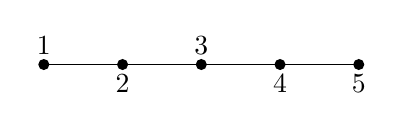
\begin{tikzpicture} [scale=1]
\coordinate [label=above:{$1$}] (1) at (-2,0);
\coordinate [label=below:{$2$}] (2) at (-1,0);
\coordinate [label=above:{$3$}] (3) at (0,0);
\coordinate [label=below:{$4$}] (4) at (1,0);
\coordinate [label=below:{$5$}] (5) at (2,0);
\fill (1) circle (2pt);
\fill (2) circle (2pt);
\fill (3) circle (2pt);
\fill (4) circle (2pt);
\fill (5) circle (2pt);
\draw (1)--(2)--(3)--(4)--(5) ;
\end{tikzpicture}
\end{center}

\item the set of available stratefies for each player is $x_i={1(Turn \ on \  the \  bulb), 0(Turn \  off \ the \  bulb)}$

\item the payoff function $u_i(x_i,x_{N_i(g)})$ of each player $i$ depends only on the action $x_i$ of player $i$ and the actions $x_{N_i(g)}$ of its neighbors $N_i(g)$, where in this case $|x_{N_i(g)}|$ is the total number of neighbors taking the action 1(Turn on the bulb).

$$u_i(x_i, x_{N_{i(g)}})=  (-1)^{I\{60 x_i+ 30 |x_{N_i(g)}|<100\}} \times \frac{(60 x_i+ 30 |x_{N_i(g)}|)}{100} $$
(Here we divided by 100 just to normalize, can do without the division, the result still holds the same.)

	\subitem For player 1 and 5: 
	$$u_i(1, 1)=-0.9$$
	$$u_i(1, 0)=-0.6$$
	$$u_i(0, 1)=-0.3$$
	$$u_i(0, 0)=0$$

$$\begin{array} {|c|c|c|c|} \hline
& \text{$|x_{N_i(g)}|=1$} & \text{$|x_{N_i(g)}|=0$}\\ \hline
\text{$x_i=1$} & -0.9 & -0.6   \\ \hline
\text{$x_i=0$} & -0.3 & 0   \\ \hline
\end{array}$$		

	\subitem For player 2,3,4: 
	$$u_i(1, 2)=1.2$$
	$$u_i(1, 1)=-0.9$$
           $$u_i(1, 0)=-0.6$$
	$$u_i(0, 2)= -0.6$$
	$$u_i(0, 1)=-0.3$$
           $$u_i(0, 0)=0$$

$$\begin{array} {|c|c|c|c|} \hline
& \text{$|x_{N_i(g)}|=2$} & \text{$|x_{N_i(g)}|=1$} & \text{$|x_{N_i(g)}|=0$}\\ \hline
\text{$x_i=1$} & 1.2 & -0.9 & -0.6   \\ \hline
\text{$x_i=0$} & -0.6 & -0.3 & 0   \\ \hline
\end{array}$$	

\end{itemize}

\item[\textbf{b.}] \textbf{(6 points)}  List any/all dominated strategies you can find in this game. \\

\textcolor{red}{Solution:}
For player 1 and 5 (at the ends of the network), 1(turn on the bulb) is the dominated strategy, since no matter what their (only) neighbor does (on or off), they would be better off by switching to 0(turn off the bulb. Intuitively, they will never be able receive 100 watts or more, their best response is to sleep and turn off their own bulb to reduce the watts, no matter what their neighbor does. 

For player ${2,3,4}$, they don't have dominated strategy. When they have two neighbors simultaneously turn on the buld, turn off the bulb is worse than turn on bulb; otherwise, turn on the bulb is worse than turn off the bulb. Therefore, there is no strategy that is always worse than the other. 



\item[\textbf{c.}] \textbf{(6 points)}  List any/all  dominant strategies you can find in this game.\\

\textcolor{red}{Solution:}
For player 1 and 5 (at the ends of the network), 0(turn off the bulb) is the dominant strategy, since no matter what their (only) neighbor does (on or off), their best response is to sleep and turn off their own bulb to reduce the watts.

For player ${2,3,4}$, they don't have dominant strategy. When they have two neighbors simultaneously turn on the buld, their best reponse is to turn on bulb and read; otherwise, their best reponse is to turn off the bulb and to sleep, for the same reasoning made for player 1 and 5, because they will never receive more than 100 watts without 2 neighbors' contribution. 


\item[\textbf{d.}] \textbf{(6 points)}   List any/all equilibria you can find in this game.\\

\textcolor{red}{Solution:} All five players turn off their own bulb.\\

Since player 1 and 5 have dominant strategy, they will surely take that action to turn off the bulb. It is equivalent to delete the dominated strategy, and we get a reduced game for player ${2,3,4}$. Now, in the reduced form, player 2 and 4 have the same situation as player 1 and 5 in the original game:

$$\begin{array} {|c|c|c|c|} \hline
& \text{$|x_{N_i(g)}|=1$} & \text{$|x_{N_i(g)}|=0$}\\ \hline
\text{$x_i=1$} & -0.9 & -0.6   \\ \hline
\text{$x_i=0$} & -0.3 & 0   \\ \hline
\end{array}$$	

Now, player 2 and 4 have dominant (and dominated) strategy, they will surely take the action to turn off the bulb. We delete player 2 and 4's dominated strategy, and get a reduced game for player 5: 

$$\begin{array} {|c|c|c|c|} \hline
 & \text{$|x_{N_i(g)}|=0$}\\ \hline
\text{$x_i=1$} & -0.6   \\ \hline
\text{$x_i=0$} & 0   \\ \hline
\end{array}$$	

Now, player 5's dominant strategy is to turn off the bulb. By IDSDS, we get the Nash equilibrium of the origianl game: All five players turn off their own bulb.

\end{itemize}
 


























\paragraph{3.} \textbf{(25 points)} Redo Exercise 2 in entirety assuming that the five strangers are seated in a round table (so that each passenger has both a right and left neighbor), instead of in a row.\\

\begin{itemize}
\item[\textbf{a.}] \textbf{(7 points)}  Transform this situation into a game (that is, list the set of players, the set of strategies and an appropriate payoff function).\\

\textcolor{red}{Solution:}

\begin{itemize}
\item the set of players $N={1,2,3,4,5}$ seat in a row, and is connected to only adjacent neighbors.
 
\begin{center}
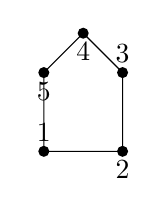
\begin{tikzpicture} [scale=1]
\coordinate [label=above:{$1$}] (1) at (0,0);
\coordinate [label=below:{$2$}] (2) at (1,0);
\coordinate [label=above:{$3$}] (3) at (1,1);
\coordinate [label=below:{$4$}] (4) at (0.5,1.5);
\coordinate [label=below:{$5$}] (5) at (0,1);
\fill (1) circle (2pt);
\fill (2) circle (2pt);
\fill (3) circle (2pt);
\fill (4) circle (2pt);
\fill (5) circle (2pt);
\draw (1)--(2)--(3)--(4)--(5)--(1);
\end{tikzpicture}
\end{center}

\item the set of available stratefies for each player is $x_i={1(Turn on the bulb), 0(Turn off the bulb)}$

\item the payoff function $u_i(x_i,x_{N_i(g)})$ of each player $i$ depends only on the action $x_i$ of player $i$ and the actions $x_{N_i(g)}$ of its neighbors $N_i(g)$, where in this case $|x_{N_i(g)}|$ is the total number of neighbors taking the action 1(Turn on the bulb).

$$u_i(x_i, x_{N_{i(g)}})=  (-1)^{I\{60 x_i+ 30 |x_{N_i(g)}|<100\}} \times \frac{(60 x_i+ 30 |x_{N_i(g)}|)}{100} $$
(Here we divided by 100 just to normalize, can do without the division, the result still holds the same.)
  
Due to symmetry, for any player $i$:
$$u_i(1, 2)=1.2$$
$$u_i(1, 1)=-0.9$$
 $$u_i(1, 0)=-0.6$$
$$u_i(0, 2)= -0.6$$
$$u_i(0, 1)=-0.3$$
 $$u_i(0, 0)=0$$

$$\begin{array} {|c|c|c|c|} \hline
& \text{$|x_{N_i(g)}|=2$} & \text{$|x_{N_i(g)}|=1$} & \text{$|x_{N_i(g)}|=0$}\\ \hline
\text{$x_i=1$} & 1.2 & -0.9 & -0.6   \\ \hline
\text{$x_i=0$} & -0.6 & -0.3 & 0   \\ \hline
\end{array}$$	

\end{itemize}

\item[\textbf{b.}] \textbf{(6 points)}  List any/all dominated strategies you can find in this game. \\

\textcolor{red}{Solution:}
For any player $i$, they don't have dominated strategy. When they have two neighbors simultaneously turn on the buld, turn off the bulb is worse than turn on bulb; otherwise, turn on the bulb is worse than turn off the bulb. Therefore, there is no strategy that is always worse than the other. 

\item[\textbf{c.}] \textbf{(6 points)}  List any/all  dominant strategies you can find in this game.\\

\textcolor{red}{Solution:}
For any player $i$, they don't have dominant strategy. When they have two neighbors simultaneously turn on the buld, their best reponse is to turn on bulb and read; otherwise, their best reponse is to turn off the bulb and to sleep, because they will never receive more than 100 watts without 2 neighbors' contribution. 


\item[\textbf{d.}] \textbf{(6 points)}   List any/all equilibria you can find in this game.\\

\textcolor{red}{Solution:} There are two NE: one with all players turn on the bulb; one with all players turn off the bulb.\\

When all players turn on the bulb, for each single player, holding all other players' strategies constant, there is no incentive to turn off the bulb, since he has 1.2 payoff versus -0.6 otherwise. When all players turn off the bulb, for each single player, holding all other players' strategies constant, there is no incentive to turn on the bulb, since he has 0 payoff versus -0.6 otherwise.

 
\end{itemize}

































\paragraph{4. Borrow-a-Book Network Game} \textbf{(30 points)} A \emph{network game} $(N, g)$ is a special class of game in which 

\begin{itemize}
\item the set of players $N$ is connected by a network $g$,
\item the set of available strategies for each player is $\{0,1\}$, and
\item the payoff function $u_i(x_i, x_{N_i(g)})$ of each player $i$ depends only on the action $x_i$ of player $i$ and the actions\footnote{$x_{N_i(g)}$ is the vector that contains all elements of $x$ that correspond to the neighbors of $i$} $x_{N_i(g)}$ of her neighbors $N_i(g)$ in the network $(N,g)$.\end{itemize}

In other words, the utility of each node is defined on both its own action and the actions of its neighbors.

Each player in a \emph{borrow-a-book network game} chooses whether to buy a book. If a player does not buy the book, then he can freely borrow it  from any of his neighbors who bought it. Indirect borrowing is not permitted, so the player cannot borrow a book from a neighbor of a neighbor. If none of a player's neighbors has bought the book, then the player would prefer to pay the cost of buying the book himself rather than not having access to the book. This is problem is a classic \emph{free rider} problem, but defined on a network. Formally:

 $$\begin{array} {l l }
u_i(1, x_{N_{i(g)}})=1-c &  \\
u_i(0, x_{N_{i(g)}})=\begin{cases}\begin{array} {l l} 1 & \text{if} \ x_j=1 \ \text{for some} \ j\in N_i(g) \\  0 & \text{if} \ x_j=0 \ \text{for all} \ j\in N_i(g)\\ \end{array}\end{cases}
\end{array}$$
 
where $1>c>0$ denotes the cost of buying the book. 

\begin{itemize}
\item[\textbf{a.}] \textbf{(5 points)} Characterize the set of Nash Equilibria of a borrow-a-book game in which the players are modeled as and linked in the form of a clique. \\

\textcolor{red}{Solution:}
For each player $i$, we can turn his payoff into a matrix as below.

$$\begin{array} {|c|c|c|c|} \hline
& \text{$|x_{N_i(g)}| \ge 1$} & \text{$|x_{N_i(g)}|=0$}\\ \hline
\text{$x_i=1$} & 1-c & 1-c  \\ \hline
\text{$x_i=0$} & 1 & 0   \\ \hline
\end{array}$$	

If at least one of his neighbors taking action 1, his best reponse is to take action 0; if none of his neighbors taking action 1, his best reponse is to take action 1. As more neighbors taking action 1, the player has less incentive to take action 1. Therefore, this is a strategic substitutive game.

In a clique network structure, the set of Nash equilibrium can be characterized as: if there are N players in the network, then there are N Nash equilibrium, in each one of them, there is only one player taking the action 1, the rest of players taking action 0. That is, only one player buys a book, and since everyone else is a friend of this player, they will all borrow the book from him. There will never have an Nash equilibrium where more than one player buying the book, because the first buyer is friend of everyone else, so nobody has the incentive to buy the book given the first player already bought the book.

For example, in a 3-player clique:
%%% example N=3
\begin{center}
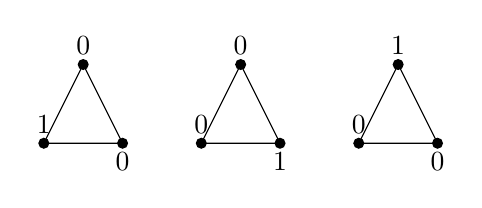
\begin{tikzpicture} [scale=1]
% example 1
\coordinate [label=above:{$1$}] (1) at (0,0);
\coordinate [label=below:{$0$}] (2) at (1,0);
\coordinate [label=above:{$0$}] (3) at (0.5,1);
\fill (1) circle (2pt);
\fill (2) circle (2pt);
\fill (3) circle (2pt);
\draw (1)--(2)--(3)--(1);
% example 2
\coordinate [label=above:{$0$}] (4) at (2,0);
\coordinate [label=below:{$1$}] (5) at (3,0);
\coordinate [label=above:{$0$}] (6) at (2.5,1);
\fill (4) circle (2pt);
\fill (5) circle (2pt);
\fill (6) circle (2pt);
\draw (4)--(5)--(6)--(4);
% example 3
\coordinate [label=above:{$0$}] (7) at (4,0);
\coordinate [label=below:{$0$}] (8) at (5,0);
\coordinate [label=above:{$1$}] (9) at (4.5,1);
\fill (7) circle (2pt);
\fill (8) circle (2pt);
\fill (9) circle (2pt);
\draw (7)--(8)--(9)--(7);
\end{tikzpicture}
\end{center}


\item[\textbf{b.}] \textbf{(5 points)}  Characterize the set of Nash Equilibria of a borrow-a-book game in which the players are modeled as and linked in the form of a ring. \\

In a ring network structure, the set of Nash equilibrium can be characterized as: starting from any player, since every player has symmetric position in a ring, say we start from player 1, let player takes the action 1, and then choose one of player 3 or 4 takes the action 1, in other words, among the players that are 2 hoops or 3 hoops away from player 1, choose one of them to take action 1 (not both), and repeat this process until the last player N, and make sure that player N could only take action 0 (since player 1 and N are neighbors). 

For example, in a 5-ring:
%%% example N=5
\begin{center}
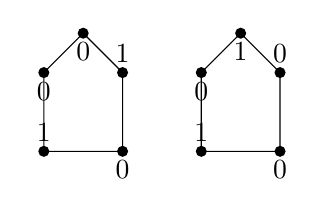
\begin{tikzpicture} [scale=1]
% example 1
\coordinate [label=above:{$1$}] (1) at (0,0);
\coordinate [label=below:{$0$}] (2) at (1,0);
\coordinate [label=above:{$1$}] (3) at (1,1);
\coordinate [label=below:{$0$}] (4) at (0.5,1.5);
\coordinate [label=below:{$0$}] (5) at (0,1);
\fill (1) circle (2pt);
\fill (2) circle (2pt);
\fill (3) circle (2pt);
\fill (4) circle (2pt);
\fill (5) circle (2pt);
\draw (1)--(2)--(3)--(4)--(5)--(1);
% example 2
\coordinate [label=above:{$1$}] (6) at (2,0);
\coordinate [label=below:{$0$}] (7) at (3,0);
\coordinate [label=above:{$0$}] (8) at (3,1);
\coordinate [label=below:{$1$}] (9) at (2.5,1.5);
\coordinate [label=below:{$0$}] (10) at (2,1);
\fill (6) circle (2pt);
\fill (7) circle (2pt);
\fill (8) circle (2pt);
\fill (9) circle (2pt);
\fill (10) circle (2pt);
\draw (6)--(7)--(8)--(9)--(10)--(6);

\end{tikzpicture}
\end{center}


\textcolor{red}{Solution:}
\item[\textbf{c.}]  \textbf{(10 points)} For any network $G$, let $m(G)$ be the minimum number of books bought in any equilibrium of the borrow-a-book game in which players are linked by $G$. Suppose we obtain $G'$ by adding some links to $G$. Is it possible that $m(G')>m(G)$? If not, (qualitatively) prove why not. If so, give an example.\\

\textcolor{red}{Solution:}
It is NOT possible that $m(G')>m(G)$. Qualitatively speaking, in a strategic substitive game, as more neighbors taking the action, the player is less likely to take the action. So adding more links to $G$, we add more friendships, so for every book buyer, they have larger influence to de-incentivize others to not buy the book. For example, in original $G$, on average, every player has 9 friends, we need 10 percent of population as minimum number of book buyers in order to achieve a Nash equilibrium; whereas in the new $G'$, on average, every player has 19 friends, we only need 5 percent of population as minimum number of book buyers in order to achieve a Nash equilibrium. In other words,  $m(G')\le m(G)$. 

 

\item[\textbf{d.}]  \textbf{(10 points)} Consider a borrow-a-book game whose players are linked by the graph $G=(N,g)$. Give a condition (or set of conditions) on the subset $N'$ of $N$ ($N'\subset N$) that precisely guarantees that the set of players $N'$ are the only ones buying the book in some equilibrium. Be as precise as possible.\\

\textcolor{red}{Solution:}
Let $N'$ be the set of players that are the only ones buying the book in some equilibrium. Any Nash equilibrium has to satisfy the conditions:
\begin{itemize}
\item each $i$ in $N'$ must have no neighbors in $N'$, i.e., all neighbors (if any) are in $N-N'$
\item each $i$ not in $N'$ (in $N-N'$) must have at least one neighbors in $N'$  
\end{itemize}




\end{itemize}


\end{document}
